\documentclass[8pt]{beamer}
\usetheme{Berkeley}
\usepackage{multicol}
\usepackage{xcolor}
\usepackage{graphicx}
\linespread{1.35}
\usepackage{amsmath}
\usepackage{color}
\usepackage{tikz}
\usetikzlibrary{arrows,automata}

\begin{document}

\begin{frame}
 \section*{Solved Problems}
\begin{flushright}
 \texttt{Finite State Machine} \hspace*{0.1cm}\textbf{$|$} \hspace*{0.1cm} \textbf{213}\hspace*{0.1cm}
\end{flushright}
\vspace*{0.5cm}

\textbf{Solution:} To retrieve the input sequence, first we need to check whether the machine is information
lossless or not. The machine is information lossless as given in Example 4.20.\\
\hspace*{0.5cm} The output successor table for the given machine is\\

\pause
\begin{center}
\begin{tabular}{ccc}
 \hline

 \hline

 \hline

 \hline
 & \multicolumn{2}{c}{$Next State, I/P$}\\
 \cline{2-3}
 $State$ &  $z=0$ & $z=1$\\
\hline
A   & (A, 0), (B, 1) &   –          \\
B   & (C, 0), (D, 1) &   –          \\
C   &  –             &(D, 0), (C, 1)\\
D   &  –             &(B, 0), (A, 1)\\
 \hline

 \hline

 \hline

 \hline
\end{tabular}
\end{center}
\end{frame}

\begin{frame}
\begin{center}
\section{picture}
\includegraphics[width=8cm,height=5cm]{213.png}
\end{center}

\hspace*{0.5cm} The final state is B, and thus the input is 01011.\\
\end{frame}

\begin{frame}
24. Design a minimal inverse of the machine shown in the following table.\\
\begin{flushright}
  [WBUT 2007, 2008]\\
\end{flushright}
  
  \pause
  \begin{center}
\begin{tabular}{ccc}
 \hline

 \hline

 \hline

 \hline
 & \multicolumn{2}{c}{$Next State$}\\
 \cline{2-3}
 $Present State$ &  $X=0$ & $X=1$\\
\hline
A & C, 0  &D, 1\\
B & D, 0  &C, 0\\
C & A, 1  &B, 1\\
D & C, 1  &D, 1\\
 \hline

 \hline

 \hline

 \hline
\end{tabular}
\end{center}

\vspace*{0.3cm}
\hspace*{0.5cm} \textbf{Solution:} To find the minimal inverse machine, fi rst we need to fi nd the order of losslessness of
the machine.\\
\end{frame}

\begin{frame}
\section*{Solved Problems}
\begin{flushleft}
    \textbf{214}\hspace*{0.1cm} \textbf{$|$} \hspace*{0.1cm} \texttt{Introduction to Automata Theory, Formal Languages and Computation}
  \end{flushleft}
  
  \vspace*{0.5cm}
    \begin{center}
\begin{tabular}{ccc}
 \hline

 \hline

 \hline

 \hline

 $Present State$ &  $z=0$ & $z=1$\\
\hline
A & C  &D \\
B & D  &C \\
C & AB & –\\
D & –  & CD \\
\hline 
AB& CD & CD \\
CD& –  &–\\
 \hline

 \hline

 \hline

 \hline
\end{tabular}
\end{center}
\hspace*{0.5cm} The testing graph is\\
\begin{center}
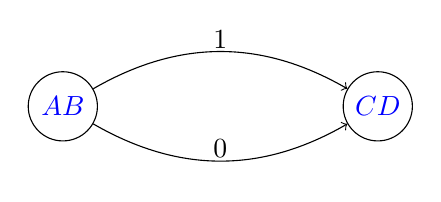
\begin{tikzpicture}[node distance = 4cm,auto,inner sep=1pt]

\node[state,text=blue,draw=black] (A)  {$AB$};
\node[state,text=blue,draw=black] (B) [right of = A]  {$CD$};

\path (A) edge [->,bend right] node {$0$} (B);
\path (A) edge [->,bend left] node {$1$} (B);

\end{tikzpicture}
\end{center}
\end{frame}

\begin{frame}
\hspace*{0.5cm} It is loop-free. And the order of finiteness is 3.\\
\hspace*{0.5cm} Therefore, if we know the initial state and the values of three successive outputs produced by
transitions from the initial state, we can determine the first input given to the machine. We need
to determine a set of triples, denoted by $\{S(t), z(t + 1)$, and $z(t + 2)\}$. There are four states of the
machine. The triples are\\

\vspace*{0.4cm}
\begin{center}

  (A, 0, 0)  \hspace*{0.3cm}  (B, 0, 1)   \hspace*{0.3cm}   (C, 0, 0)    \hspace*{0.3cm}   (D, 1, 0)\\
  (A, 1, 1)  \hspace*{0.3cm}  (B, 1, 0)   \hspace*{0.3cm}   (C, 0, 1)    \hspace*{0.3cm}   (D, 1, 1)\\

\end{center}
\end{frame}

\begin{frame}
\begin{center}
\begin{tabular}{ccc}
 \hline

 \hline

 \hline

 \hline
 & \multicolumn{2}{c}{$Next State,X$}\\
 \cline{2-3}
 $Present State$ &  $z=0$ & $z=1$\\
\hline
(A, 0, 0)  &  (C, 0, 0), 0  &  (C, 0, 1), 0\\
(A, 1, 1)  &  (D, 1, 0), 1  &  (D, 1, 1), 1\\
(B, 0, 1)  &  (D, 1, 0), 0  &  (D, 1, 1), 0\\
(B, 1, 0)  &  (C, 0, 0), 1  &  (C, 0, 1), 1\\
(C, 0, 0)  &  (A, 0, 0), 0  &  (B, 0, 1), 1\\
(C, 0, 1)  &  (B, 1, 0), 1  &  (A, 1, 1), 0\\
(D, 1, 0)  &  (C, 0, 0), 0  &  (C, 0, 1), 0\\
(D, 1, 1)  &  (D, 1, 0), 1  &  (D, 1, 1), 1\\
 \hline

 \hline

 \hline

 \hline
\end{tabular}
\end{center}

\vspace*{0.4cm}
\hspace*{0.5cm} Here, states (A, 0, 0), (D, 1, 0) and (A, 1, 1) and (D, 1, 1) are equivalent states as they produce
the same next state and same output. Let us assign $(A, 0, 0)$ as $S_1, (A, 1, 1)$ as $S_2, (B, 0, 1)$ as $S_3,
(B, 1, 0)$ as $S4, (C, 0, 0)$ as $S_5$, and $(C, 0, 1)$ as $S_6$.\\
\end{frame}

\begin{frame}
 \section*{Multiple Choice Questions}
\begin{flushright}
 \texttt{Finite State Machine} \hspace*{0.1cm}\textbf{$|$} \hspace*{0.1cm} \textbf{215}\hspace*{0.1cm}
\end{flushright}
\vspace*{1cm}

\hspace*{0.5cm} The minimal inverse machine is\\

\vspace*{0.5cm}
\begin{center}
\begin{tabular}{ccc}
 \hline

 \hline

 \hline

 \hline
 & \multicolumn{2}{c}{$Next State,X$}\\
 \cline{2-3}
 $Present State$ &  $z=0$ & $z=1$\\
\hline
$S_1$    &  $S_5, 0$   &  $S6, 0$ \\
$S_2$    &  $S_1, 1$   &  $S2, 1$ \\
$S_3$    &  $S_1, 0$   &  $S2, 0$ \\
$S_4$    &  $S_5, 1$   &  $S6, 1$ \\
$S_5$    &  $S_1, 0$   &  $S3, 1$ \\
$S_6$    &  $S_4, 1$   &  $S2, 0$ \\
 \hline

 \hline

 \hline

 \hline
\end{tabular}
\end{center}

\vspace*{0.4cm}
\end{frame}

\begin{frame}
\begin{center}
\section{picture}
\includegraphics[width=11cm,height=0.5cm]{215.png}
\end{center}

\begin{multicols}{2}
1. A palindrome cannot be recognized by any
FSM because\\
\hspace*{0.4cm} a) An FSM cannot remember arbitrary,
large amount of information\\
\hspace*{0.4cm} b) An FSM cannot deterministically fix
the mid-point\\
\hspace*{0.4cm} c) Even if the mid-point is known, an
FSM cannot find whether the second
half of the string matches the first half\\
\hspace*{0.4cm} d) All of these\\

\vspace*{0.3cm}
2. The basic limitation of an FSM is that\\
\hspace*{0.4cm} a) It cannot remember arbitrary, large
amount of information\\
\hspace*{0.4cm} b) It cannot recognize grammars that are
regular\\
\hspace*{0.4cm} c) It sometimes recognizes grammars that
are not regular\\
\hspace*{0.4cm} d) All of these\\

\vspace*{0.3cm} 
3. The operation of synchronous circuits are
controlled by\\
\hspace*{0.4cm} a) Input\\
\hspace*{0.4cm} b) State\\
\hspace*{0.4cm} c) Output\\
\hspace*{0.4cm} d) Clock pulses\\

\vspace*{0.3cm}
4. The output of combinational circuit depends
on\\
\hspace*{0.4cm} a) Present state\\
\hspace*{0.4cm} b) Past input\\
\hspace*{0.4cm} c) Present input\\
\hspace*{0.4cm} d) Present stored information and present
input\\
\end{multicols}
\end{frame}

\begin{frame}
\begin{multicols}{2}
5. The output of sequential circuit depends on\\
\hspace*{0.4cm} a) Present state\\
\hspace*{0.4cm} b) Past input\\
\hspace*{0.4cm} c) Present input\\
\hspace*{0.4cm} d) Present stored information and present
input\\

\vspace*{0.3cm}
6. For which of the following, FSM cannot be
designed\\
\hspace*{0.4cm} a) Addition of two binary numbers\\
\hspace*{0.4cm} b) Subtraction of two binary numbers\\
\hspace*{0.4cm} c) Multiplication of two binary numbers\\
\hspace*{0.4cm} d) All of these\\

\vspace*{0.3cm}
7. Which is true of the following?\\
\hspace*{0.4cm} a) A merger graph is a directed graph\\
\hspace*{0.4cm} b) A compatible graph is a directed graph\\
\hspace*{0.4cm} c) Both are not directed\\
\hspace*{0.4cm} d) None of these\\

\vspace*{0.3cm}
8. A merger table is a substitute of\\
\hspace*{0.4cm} a) Merger graph\\
\hspace*{0.4cm} b) Compatible graph\\
\hspace*{0.4cm} c) Minimized machine\\
\hspace*{0.4cm} d) FSM\\

\vspace*{0.3cm}
9. Two states are called 1-equivalent if\\
\hspace*{0.4cm} a) Both of the states produce 1\\
\hspace*{0.4cm} b) If both of the states produce the same
output for string length 1\\
\end{multicols}
\end{frame}

\begin{frame}
\section*{Multiple Choice Questions}
\begin{flushleft}
    \textbf{216}\hspace*{0.1cm} \textbf{$|$} \hspace*{0.1cm} \texttt{Introduction to Automata Theory, Formal Languages and Computation}
  \end{flushleft}

  \vspace*{0.5cm}
\begin{multicols}{2}
\hspace*{0.4cm} c) If both of the states produce the same
output for same input.\\
\hspace*{0.4cm} d) If both of the states produce the same
output for input 1.\\

\vspace*{0.3cm}
10. Which is true for an incompletely specified
machine?\\
\hspace*{0.4cm} a) All Next states are not mentioned\\
\hspace*{0.4cm} b) All outputs are not mentioned\\
\hspace*{0.4cm} c) All inputs are not mentioned\\
\hspace*{0.4cm} d) Both a and b\\

\vspace*{0.3cm}
11. Compatible pairs are obtained from
\hspace*{0.4cm} a) Merger graph\\
\hspace*{0.4cm} b) Compatible graph\\
\hspace*{0.4cm} c) Testing table\\
\hspace*{0.4cm} d) Testing graph\\

\vspace*{0.3cm}
12. The number of vertices of a merger graph is\\
\hspace*{0.4cm} a) The number of states of the machine\\
\hspace*{0.4cm} b) The number of compatible pairs\\
\hspace*{0.4cm} c) The number of states combinations\\
\hspace*{0.4cm} d) None of these\\

\vspace*{0.3cm}
13. The number of vertices of a compatible
graph is\\
\hspace*{0.4cm} a) The number of states of the machine\\
\hspace*{0.4cm} b) The number of compatible pairs\\
\hspace*{0.4cm} c) The number of states combinations\\
\hspace*{0.4cm} d) None of these\\
\end{multicols}
\end{frame}

\begin{frame}
\begin{multicols}{2}
14. An FSM M is called a finite memory
machine of order $\mu$ if the present state of the
machine M can be obtained from\\
\hspace*{0.4cm} a) The last $\mu$ number of inputs and the
corresponding $\mu$ number of next states\\
\hspace*{0.4cm} b) The last $\mu$ number of inputs and the
corresponding $\mu$ number of outputs\\
\hspace*{0.4cm} c) The last $\mu$ number of next states and the
corresponding $\mu$ number of outputs\\
\hspace*{0.4cm} d) The last $\mu$ number of inputs\\

\vspace*{0.3cm}
15. A sequential machine M is called definite if
there exists a least integer $\mu$, so that the present
state of the machine M can be uniquely
obtained from the\\
\hspace*{0.4cm} a) Past $\mu$ number of inputs\\
\hspace*{0.4cm} b) Past $\mu$ number of outputs\\
\hspace*{0.4cm} c) Past $\mu$ number of next states\\
\hspace*{0.4cm} d) Past $\mu$ number of inputs, outputs, and
next states\\

\vspace*{0.3cm}
16. Which is sufficient to find the initial state
of an information lossless machine from the
input string?\\
\hspace*{0.4cm} a) Next state and output string\\
\hspace*{0.4cm} b) Final state and next state\\
\hspace*{0.4cm} c) Final state and output string\\
\hspace*{0.4cm} d) Final state, next state, and output string\\



\end{multicols}

\vspace*{0.3cm}
\end{frame}


\begin{frame}
\begin{multicols}{2}

17. The input sequence of an information lossless
machine can be determined from the
knowledge of\\
\hspace*{0.4cm} a) Only the output sequence\\
\hspace*{0.4cm} b) The output sequence and initial state\\
\hspace*{0.4cm} c) The output sequence, initial state, and
final state\\
\hspace*{0.4cm} d) The initial state\\

\vspace*{0.3cm}
18. Which is true of the following?
\hspace*{0.4cm} a) All information lossless machines are
of finite order\\
\hspace*{0.4cm} b) Some information lossless machines
are of finite order\\
\hspace*{0.4cm} c) Those machines which are not lossless
of finite order are lossy\\
\hspace*{0.4cm} d) None of the above\\

\vspace*{0.3cm}
19. The following diagram represents an FSM
which takes as input a binary number from
the least significant bit.\\
\begin{center}
\section{picture}
\includegraphics[width=4cm,height=2cm]{216.png}
\end{center}
\hspace*{0.4cm} Which one of the following is true?\\
\hspace*{0.4cm} (a) It computes 1's complement of the
input number\\
\hspace*{0.4cm} (b) It computes 2's complement of the
input number\\
\hspace*{0.4cm} (c) It increments the input number\\
\hspace*{0.4cm} (d) It decrements the input number\\
\end{multicols}
\end{frame}

\end{document}